\subsection{Grafikus adattárolás (vektor, raszter), alkatrész modellezési módszerek.}

\textbf{Adattárolási stratégiák elvei:}
\begin{center}
    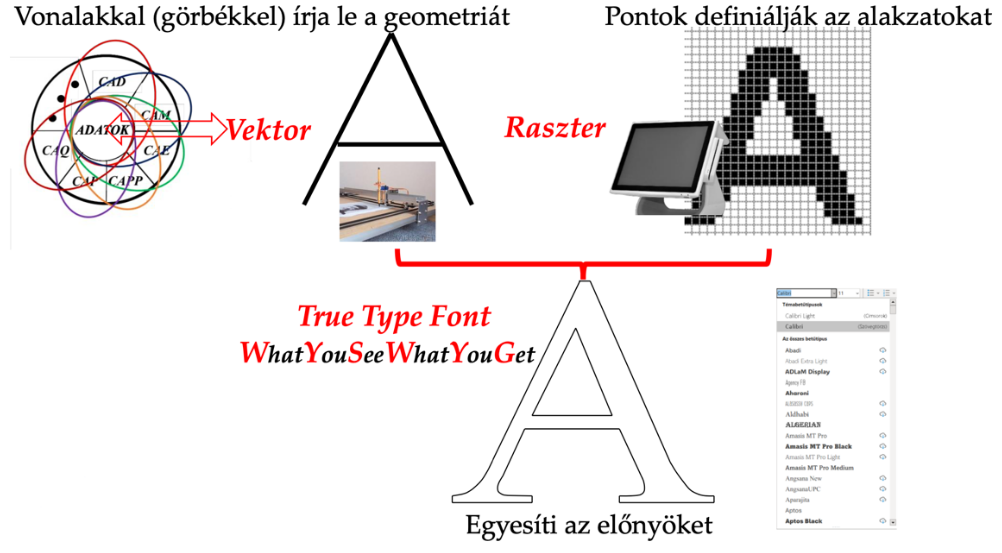
\includegraphics[width=0.9\textwidth]{res/imgs/info_20_storage_strategies.png}
\end{center}

\textbf{Vektoros adattárolás:}
\begin{itemize}
    \item lineáris lista:
\end{itemize}
\begin{center}
    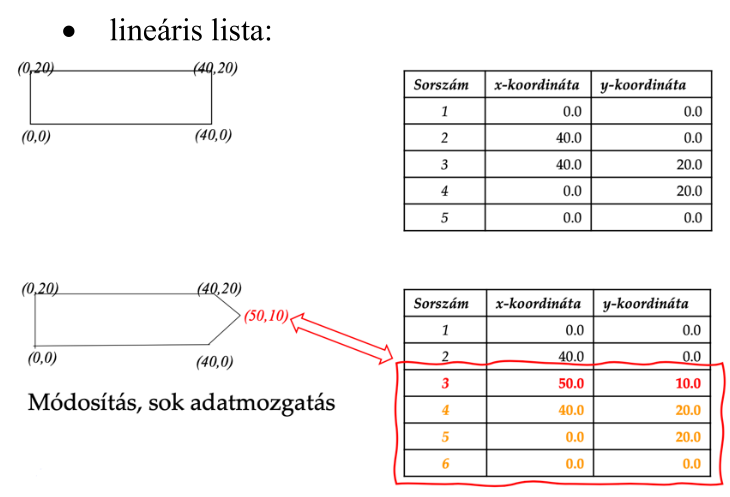
\includegraphics[width=0.8\textwidth]{res/imgs/info_20_linear_list.png}
\end{center}
Módosítás, sok adatmozgatás

\begin{itemize}
    \item láncolt lista:
\end{itemize}
\begin{center}
    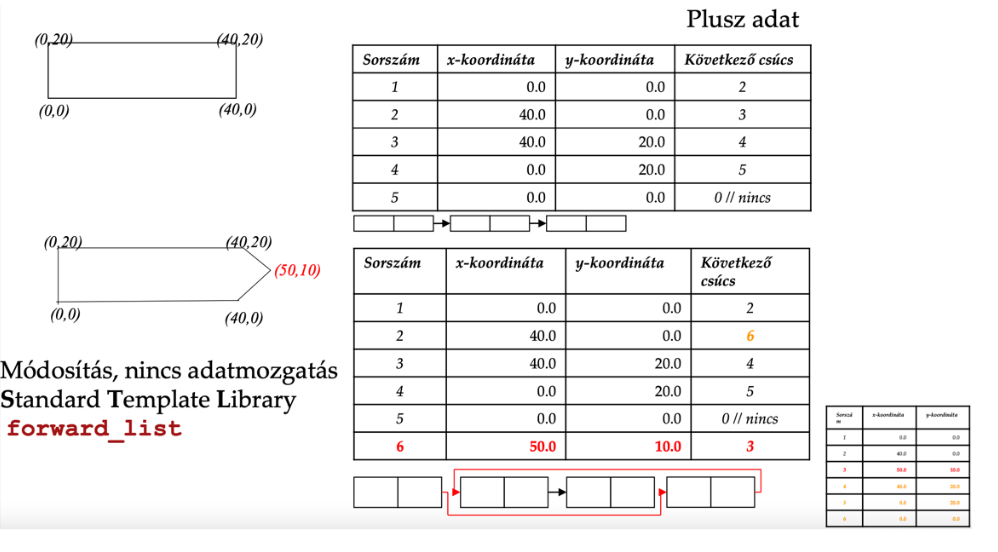
\includegraphics[width=0.8\textwidth]{res/imgs/info_20_linked_list.png}
\end{center}
Módosítás, nincs adatmozgatás. Standard Template Library \texttt{forward\_list}

\begin{itemize}
    \item keresztláncolt lista:
\end{itemize}
\begin{center}
    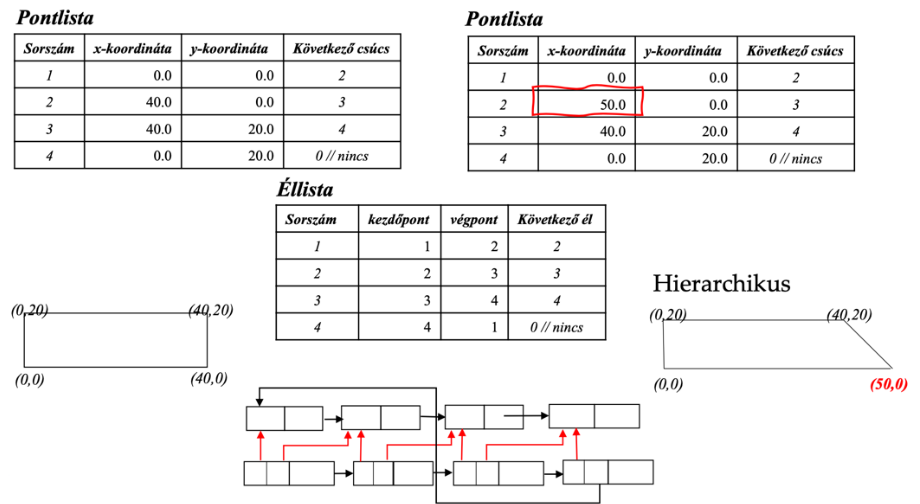
\includegraphics[width=0.9\textwidth]{res/imgs/info_20_cross_linked.png}
\end{center}

\textbf{Raszteres adattárolás:}
\begin{itemize}
    \item bitkép:
    \begin{center}
        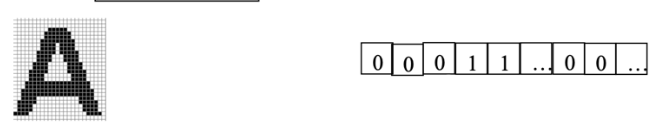
\includegraphics[width=0.6\textwidth]{res/imgs/info_20_bitmap.png}
    \end{center}
    \item 4-es fa:
    \begin{center}
        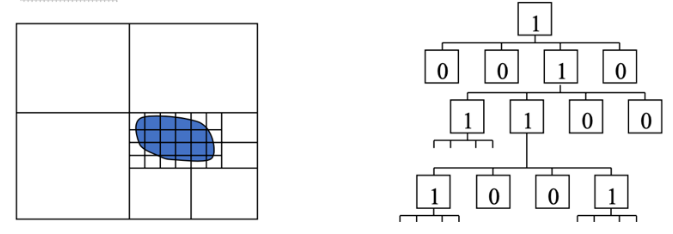
\includegraphics[width=0.7\textwidth]{res/imgs/info_20_quadtree.png}
    \end{center}
    \item 8-as fa:
    \begin{center}
        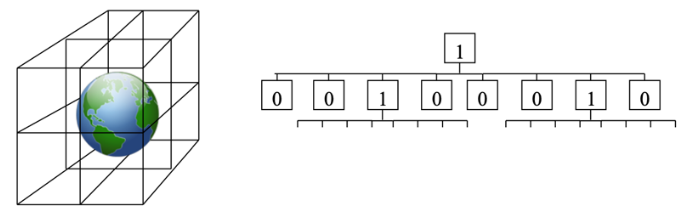
\includegraphics[width=0.8\textwidth]{res/imgs/info_20_octree.png}
    \end{center}
\end{itemize}

\textbf{Modellezési módszerek:}
\begin{center}
    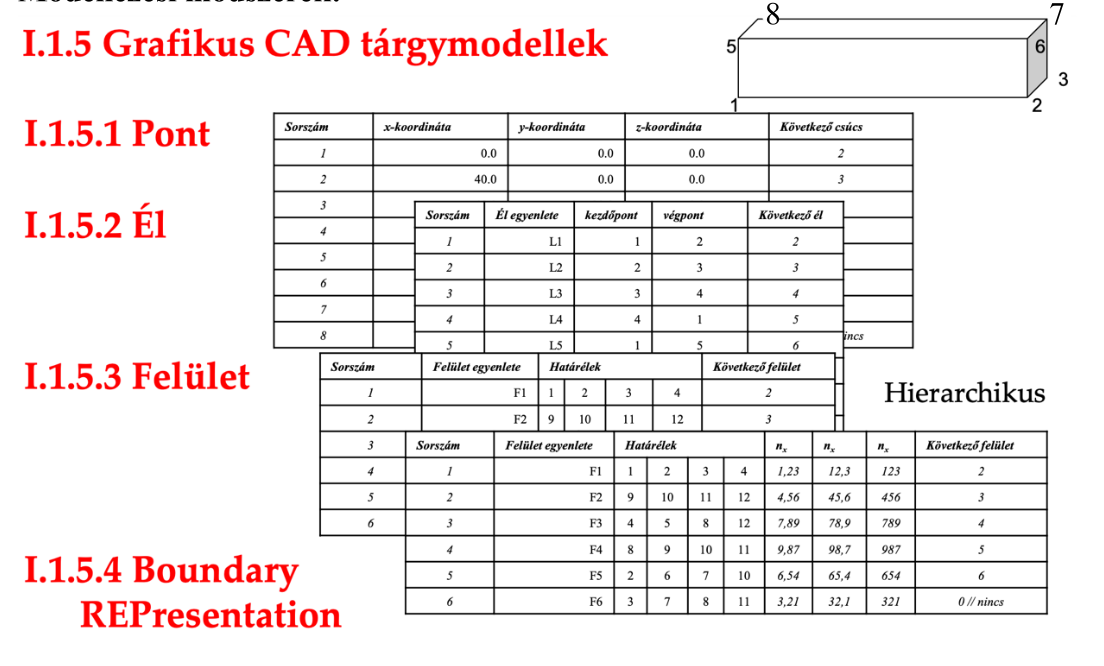
\includegraphics[width=0.95\textwidth]{res/imgs/info_20_cad_models.png}
\end{center}
\begin{center}
    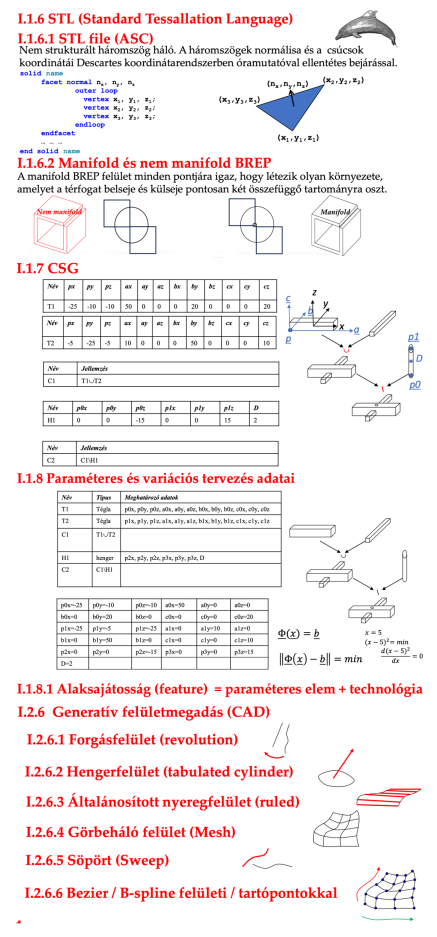
\includegraphics[width=0.95\textwidth]{res/imgs/info_20_cad_models_2.png}
\end{center}